% -*- coding: utf-8 -*-
%-------------------------designed by zcf--------------
\documentclass[UTF8,a4paper,10pt]{ctexart}
\usepackage[left=3.17cm, right=3.17cm, top=2.74cm, bottom=2.74cm]{geometry}
\usepackage{amsmath}
\usepackage{graphicx,subfig}
\usepackage{float}
\usepackage{cite}
\usepackage{caption}
\usepackage{enumerate}
\usepackage{booktabs} %表格
\usepackage{multirow}
\newcommand{\tabincell}[2]{\begin{tabular}{@{}#1@{}}#2\end{tabular}}  %表格强制换行
%-------------------------字体设置--------------
% \usepackage{times} 
\usepackage{ctex}
\setCJKmainfont[ItalicFont=Noto Sans CJK SC Bold, BoldFont=Noto Serif CJK SC Black]{Noto Serif CJK SC}


\newcommand{\yihao}{\fontsize{26pt}{36pt}\selectfont}           % 一号, 1.4 倍行距
\newcommand{\erhao}{\fontsize{22pt}{28pt}\selectfont}          % 二号, 1.25倍行距
\newcommand{\xiaoer}{\fontsize{18pt}{18pt}\selectfont}          % 小二, 单倍行距
\newcommand{\sanhao}{\fontsize{16pt}{24pt}\selectfont}  %三号字
\newcommand{\xiaosan}{\fontsize{15pt}{22pt}\selectfont}        % 小三, 1.5倍行距
\newcommand{\sihao}{\fontsize{14pt}{21pt}\selectfont}            % 四号, 1.5 倍行距
\newcommand{\banxiaosi}{\fontsize{13pt}{19.5pt}\selectfont}    % 半小四, 1.5倍行距
\newcommand{\xiaosi}{\fontsize{12pt}{18pt}\selectfont}            % 小四, 1.5倍行距
\newcommand{\dawuhao}{\fontsize{11pt}{11pt}\selectfont}       % 大五号, 单倍行距
\newcommand{\wuhao}{\fontsize{10.5pt}{15.75pt}\selectfont}    % 五号, 单倍行距
%-------------------------章节名----------------
\usepackage{ctexcap} 
\CTEXsetup[name={,、},number={ \chinese{section}}]{section}
\CTEXsetup[name={(,)},number={\chinese{subsection}}]{subsection}
\CTEXsetup[name={,.},number={\arabic{subsubsection}}]{subsubsection}
%-------------------------页眉页脚--------------
\usepackage{fancyhdr}
\pagestyle{fancy}
\lhead{\kaishu \leftmark}
% \chead{}
\rhead{\kaishu 计算机网络实验报告}
\lfoot{}
\cfoot{\thepage}
\rfoot{}
\renewcommand{\headrulewidth}{0.1pt}  
\renewcommand{\footrulewidth}{0pt}%去掉横线
\newcommand{\HRule}{\rule{\linewidth}{0.5mm}}%标题横线
\newcommand{\HRulegrossa}{\rule{\linewidth}{1.2mm}}
%-----------------------伪代码------------------
\usepackage{algorithm}  
\usepackage{algorithmicx}  
\usepackage{algpseudocode}  
\floatname{algorithm}{Algorithm}  
\renewcommand{\algorithmicrequire}{\textbf{Input:}}  
\renewcommand{\algorithmicensure}{\textbf{Output:}} 
\usepackage{lipsum}  
\makeatletter
\newenvironment{breakablealgorithm}
  {% \begin{breakablealgorithm}
  \begin{center}
     \refstepcounter{algorithm}% New algorithm
     \hrule height.8pt depth0pt \kern2pt% \@fs@pre for \@fs@ruled
     \renewcommand{\caption}[2][\relax]{% Make a new \caption
      {\raggedright\textbf{\ALG@name~\thealgorithm} ##2\par}%
      \ifx\relax##1\relax % #1 is \relax
         \addcontentsline{loa}{algorithm}{\protect\numberline{\thealgorithm}##2}%
      \else % #1 is not \relax
         \addcontentsline{loa}{algorithm}{\protect\numberline{\thealgorithm}##1}%
      \fi
      \kern2pt\hrule\kern2pt
     }
  }{% \end{breakablealgorithm}
     \kern2pt\hrule\relax% \@fs@post for \@fs@ruled
  \end{center}
  }
\makeatother
%------------------------代码-------------------
\usepackage{xcolor} 
\usepackage{listings} 
\usepackage{graphicx}
\lstset{ 
breaklines,%自动换行
basicstyle=\small,
escapeinside=``,
keywordstyle=\color{ blue!70} \bfseries,
commentstyle=\color{red!50!green!50!blue!50},% 
stringstyle=\ttfamily,% 
extendedchars=false,% 
linewidth=\textwidth,% 
numbers=left,% 
numberstyle=\tiny \color{blue!50},% 
frame=trbl% 
rulesepcolor= \color{ red!20!green!20!blue!20} 
}
%------------超链接----------
\usepackage[colorlinks,linkcolor=black,anchorcolor=blue]{hyperref}
%------------------------TODO-------------------
\usepackage{enumitem,amssymb}
\newlist{todolist}{itemize}{2}
\setlist[todolist]{label=$\square$}
% for check symbol 
\usepackage{pifont}
\newcommand{\cmark}{\ding{51}}%
\newcommand{\xmark}{\ding{55}}%
\newcommand{\done}{\rlap{$\square$}{\raisebox{2pt}{\large\hspace{1pt}\cmark}}\hspace{-2.5pt}}
\newcommand{\wontfix}{\rlap{$\square$}{\large\hspace{1pt}\xmark}}
%------------------------水印-------------------
\usepackage{tikz}
\usepackage{xcolor}
\usepackage{eso-pic}
\usepackage{verbatim}

\newcommand{\watermark}[3]{\AddToShipoutPictureBG{
\parbox[b][\paperheight]{\paperwidth}{
\vfill%
\centering%
\tikz[remember picture, overlay]%
  \node [rotate = #1, scale = #2] at (current page.center)%
    {\textcolor{gray!80!cyan!30!magenta!30}{#3}};
\vfill}}}
\lstset{
  basicstyle=\ttfamily\small, % 使用打字机字体并设置为小号
  numbers=left,
}
%———————————————————————————————————————————正文
%----------------------------------------------
\begin{document}
\begin{titlepage}
    \begin{center}
    
\includegraphics[width=0.8\textwidth]{NKU.png}\\[1cm]    
    \textsc{\Huge \kaishu{\textbf{南\ \ \ \ \ \ 开\ \ \ \ \ \ 大\ \ \ \ \ \ 学}} }\\[0.9cm]
    \textsc{\huge \kaishu{\textbf{网\ \ 络\ \ 空\ \ 间\ \ 安\ \ 全\ \ 学\ \ 院}}}\\[0.9cm]
    \textsc{\huge \kaishu{\textbf{计算机网络实验报告}}}\\[0.8cm]
    \HRule \\[0.9cm]
    { \LARGE \bfseries Lab3-1 基于UDP的可靠传输}\\[0.4cm]
    \HRule \\[2.0cm]
    \centering
    \textsc{\LARGE \kaishu{2113946\ \ \ 刘国民 }}\\[0.5cm]
    \textsc{\LARGE \kaishu{年级\ :\ 2021级}}\\[0.5cm]
    \textsc{\LARGE \kaishu{专业\ :\ 信息安全}}\\[0.5cm]
    \vfill
    {\Large \today}
    \end{center}
\end{titlepage}



\newpage
\tableofcontents
\setcounter{page}{1}

\vspace{1cm}

\section{实验内容}
本次实验利用数据报套接字在用户空间实现面向连接的可靠数据传输,功能包括:建立连接、差错检测、接收确认、超时重传等。流量控制采用停等机制,完成给定测试文件的传输。
\vspace{1cm}

\section{协议设计}
协议设计分为报文格式、差错检验、建立连接、数据传输和关闭连接五个部分来。
\subsection{报文格式}
本次实验中采用以下结构的数据报:
\begin{lstlisting}[frame=trbl,language={C++}]
struct Datagram {
    bool ack, syn, fin;
    uint16_t checksum;//16位校验和
    long long seqnum, acknum;
    int DataLen;// DataLen<=MaxBufferSize
    char data[MaxBufferSize] = { 0 };
}SendData, ReceiveData;
\end{lstlisting}
为实现可靠传输,在利用UDP服务发送数据时,我们将原始数据缓冲区与ack,syn,fin等标志位和校验和等信息封装在一个结构体中用于实际传输。按照结构体的定义以及C++语言内存对齐的特性,可以得到一个数据报的大小为4128字节。下面对结构体中各个成员进行说明:\par
\begin{itemize}
\item ack:用于表示是否为ack数据报,用于建立、关闭连接以及数据确认中。
\item syn:用于表示是否为syn数据报,建立连接时使用。
\item fin:用于表示是否为fin数据报,关闭连接时使用,
\item checksum:十六位校验和,用于指示传输过程中数据是否丢失或者被错误更改。
\item seqnum:发送序列号,指示当前传输数据的字节序号
\item acknum:发送序列号,指示收到数据的字节序号
\item DataLen:实际传输的数据大小(以字节为单位)。
\item data[MaxBufferSize]:数据缓冲区,用于填充发送或者接收的数据。
\end{itemize}

\subsection{差错检验}
差错检验使用以下算法实现:
\begin{enumerate}
    \item 将数据报按16bit为一组进行分组,不足一组的用0补齐
    \item 将checksum字段置0
    \item 按位累加所有组的值,每次相加如果最高位有溢出则补到16位数的最低位上
    \item 将上述步骤的结果取反后填入checksum字段
\end{enumerate}\par
接收方拿到数据后,仍按照上述算法计算校验和,但最后一步无需取反,最后再将计算出的校验和与接收数据的原checksum字段相加,若为0xffff则代表传输无误。在传输过程中,如果数据报出现差错,那么最后计算出的校验和与原始校验和相加后,则不为0xfffff。校验和的核心思想即是将所有的传输数据进行累加计算,通过比较传输前后的数值来判断传输是否出现差错。而一旦有一个或者多个比特位出现错误,最后计算得到的结果和原始校验和都会有差异。同时通过取反的方式,能够加快校验过程,避免逐比特位的比对。

\subsection{建立连接}
本次实验中采用类似TCP三次握手的方式来建立连接。如下图所示:
\begin{figure}[H]
    \centering
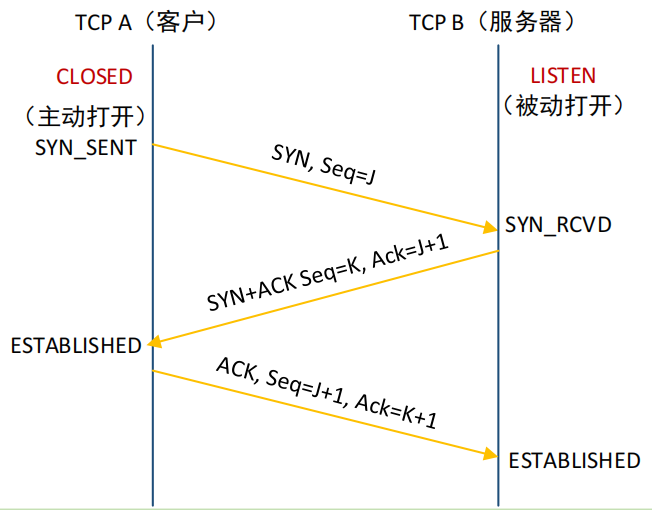
\includegraphics[width=0.6\textwidth]{img/建立连接.png}
    \caption{建立连接}
\end{figure}
在三次挥手建立连接时,不采用超时重传机制,但仍用校验和进行差错检查。如果发送的数据包有误或者丢失,则连接失败,重新打开程序尝试连接。建立连接的详细步骤如下所示:
\begin{enumerate}
    \item 首先发送方发送一个空数据报给接收方(全为0),仅将syn标志位置为1,表示发送方请求建立连接。同时阻塞等待接收方的syn+ack包。
    \item 接收方持续阻塞等待发送方的syn包,如果成功接收到syn标志位为1的数据包,则将一个空包的syn、ack和acknum位置为1后发回,告诉发送方成功收到seqnum为0的syn包。
    \item 发送方成功收到syn+ack包后,发回一个ack包,同时设置seqnum和acknum为1,表示成功收到seqnum为0的syn+ack包,同时序列号自增1。至此连接建立完成,
\end{enumerate}\par
从以上步骤可以看到,与图示步骤相对比,在这里我们让图中的初始序列号J、K均为0,最后第三次握手发送方发给接收方的ack包的seqnum和acknum均为1。以上步骤双方采用recvfrom阻塞的方式进行,如果收到的数据报有误或者丢失,则建立连接失败,重启程序重新建立连接。

\subsection{传输数据}
\subsubsection{停等机制}
对于发送方,实际传输文件时使用的初始序列号为2,每次传输时在DataLen字段填入数据缓冲区实际的数据大小,下一次传输的序列号则用当前序列号加上本次传输的数据大小。发出数据包后,发送方将等待接收方发回的ack包。下面列出不同情形下所对应的操作:
\begin{itemize}
    \item 首先进行校验和检验,如果错误则重传数据包
    \item 检验无误后判断acknum是否为下一次传输的序列号,判断ack字段是否为1,如果不相等或者不为1则重传数据包
    \item 设置最大重传次数(本次实验中设为5),如果重传超过五次,则直接关闭连接,终止传输。
\end{itemize}\par
\vspace{1cm}
对于接收方收到的数据包,进行的操作相对复杂和繁琐,下面列出不同情形下所对应的操作:
\begin{itemize}
    \item 首先需要进行校验和检验,如果错误则直接丢弃,继续等待下一个数据包
    \item 接收方需要维护一个期望序列号变量。如果收到的数据包的序列号不等于期望序列号,则说明收到的数据包失序,在这里也是直接丢弃,等待下一个数据包。(后续实验中可以考虑在这里引入乱序缓存和选择重传机制)
    \item 如果符合期望,则回复一个ack包给发送端,ack包不需要设置传输序列号(置为0),只需要将acknum设置为传输数据的大小和传输序列号之和(也就是发送端下一次将要发送的序列号),代表在此之前的数据都已确认收到。
    \item 用一个变量来维护上一次接收数据包的序列号,如果本次接收的序列号等于上一次的序列号,说明上一次传输中,接收方收到了序号正确的数据包,但发回的ack包丢失或者超时,导致发送方重传数据。在此情况下不写入文件,避免重复写入数据;反之则将收到的数据写入文件中。
\end{itemize}\par
每次回复ack报文时,,然后发回给发送方。发送方在recvfrom等待接收方的ack包时,需要验证acknum是否为该值。如果出现乱序的情况,则重发数据包。通过以上设计,原本无序的UDP数据包能够按照发出的先后顺序,依次到达接收端。

\subsubsection{超时重传}
建立连接后,发送方将recvfrom设置为非阻塞模式,同时设置阻塞时间为1000(毫秒),如果在阻塞时间之内没有收到数据包,则recvfrom将停止阻塞并返回错误码。

基于上述机制,我们可以在UDP无序或者乱序的传输服务基础上,实现基本的可靠传输。在后续实验中,会逐步考虑传输性能问题,用GBN、选择重传等机制来提高传输效率。


\subsection{关闭连接}
关闭连接使用与TCP四次挥手相类似的流程。
\begin{figure}[H]
    \centering
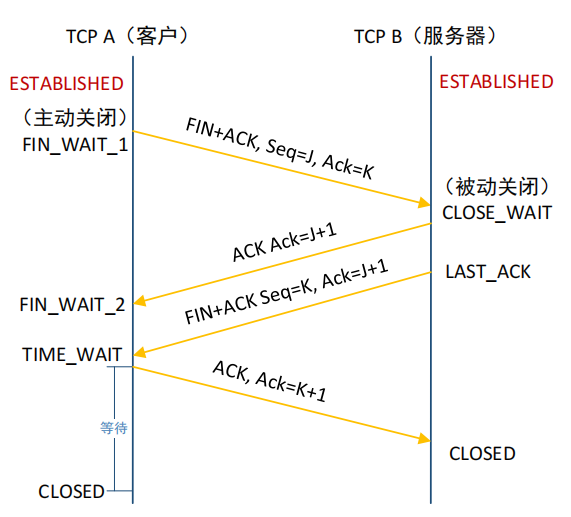
\includegraphics[width=0.6\textwidth]{img/关闭连接.png}
    \caption{关闭连接}
\end{figure}
如上图所示,但序列号J和K在此处跟三次握手类似,均取为0。

\section{代码实现}
按照协议设计中给出的一系列机制和方法,我们用代码实现了UDP上的可靠传输,并成功完成样例文件的传输,下面对部分核心代码片段进行分析。
\subsection{发送端}
\begin{lstlisting}[frame=trbl,language={C++}]
struct Datagram {
    bool ack, syn, fin;
    uint16_t checksum;//16位校验和
    long long seqnum, acknum;
    int DataLen;// DataLen<=MaxBufferSize
    char data[MaxBufferSize] = { 0 };
}SendData, ReceiveData;
\end{lstlisting}\par
上述定义的SendData和ReceiveData用于存储要发送或者要接收的数据,会在后续的Send和Receive函数中调用。每次发送/接收数据时,现将结构体变量清0然后调用sendto或者recvfrom函数。通过这种方式,可以避免传输数据时重复定义数据包。\par
差错检验代码如下:
\begin{lstlisting}[frame=trbl,language={C++}]
uint16_t Checksum(Datagram d,int flag) {
    unsigned short* check = (unsigned short*)&d;//两字节为一组来处理
    int count = DatagramLen / sizeof(short);// 一个数据报有 count组
    // 一共4128字节,能够被16比特(2字节)整除,故无需填充0
    d.checksum = 0;
    unsigned long sum = 0;
    while (count--) {
        sum += *check;
        check++;
        if (sum & 0xffff0000) {// 最高位有溢出
            sum = sum & 0xffff;
            sum++;
        }
    }
    if (flag == SEND_CHECK) {
        return (~sum) & 0xffff;//取反
    }
    else{
        return sum & 0xffff;
    }
}
\end{lstlisting}\par
在以上代码中,short指针以16bit为一组对struct结构体进行处理。由于一个结构体是4128个字节,能够被2字节(16bit)整除,所以无需填0。之后按照给出的算法,移动check指针来不断获取16位数并累加到sum变量上,通过与掩码0xffff0000相与判断最高位是否有溢出,有溢出则sum++。在这里,SEND\_CHECK是预定义的宏,用于区分是在send还是receive得时候计算校验和,如果是send则需要取反。\par

\begin{lstlisting}[frame=trbl,language={C++}]
void init() {
    WSADATA wsaData = { 0 };
    int err;
    err = WSAStartup(MAKEWORD(2,2), &wsaData);
    if (err == SOCKET_ERROR) {
        cout << "打开WSA失败!" << endl;
    }
    SenderSocket = socket(AF_INET, SOCK_DGRAM, IPPROTO_UDP);
    if (SenderSocket == SOCKET_ERROR) {
        cout << "打开套接字失败!" << endl;
    }
    
    Receiver_addr.sin_family = AF_INET; //地址类型
    Receiver_addr.sin_addr.S_un.S_addr = inet_addr("127.0.0.1"); //地址
    Receiver_addr.sin_port = htons(RouterPort); //端口号

    Sender_addr.sin_family = AF_INET; //地址类型
    Sender_addr.sin_addr.S_un.S_addr = inet_addr("127.0.0.1"); //地址
    Sender_addr.sin_port = htons(SenderPort); //端口号
    bind(SenderSocket, (LPSOCKADDR)&SenderSocket, sizeof(Sender_addr));

    cout << "发送方初始化成功!" << endl;
}
\end{lstlisting}\par
初始化函数主要完成Socket编程的初始化操作,包括打开Socket套接字,设置地址和端口号等常规操作,注意Socket套接字需要设置成 SOCK\_DGRAM 数据报模式,并使用UDP服务。\par

\begin{lstlisting}[frame=trbl,language={C++}]
bool Receive() {// 超时或者数据有误时返回false
    int len = sizeof(Receiver_addr);
    if (SOCKET_ERROR == recvfrom(SenderSocket, (char*)&ReceiveData, DatagramLen, 0,
        (struct sockaddr*)&Receiver_addr, &len)) {
        if (WSAGetLastError()== WSAETIMEDOUT) {
            cout << "接收超时!" << endl;
        }
        else {
            cout << "接受失败!" << endl;
        }
        return false;
    }
    int check = Checksum(ReceiveData, RECEIVE_CHECK);
    if ((check ^ ReceiveData.checksum) == 0xffff) {// 数据无误
        return true;
    }
    else return false;
}
\end{lstlisting}\par
Receive函数将差错检验和recvfrom封装在了一起,同时返回一个bool类型的返回值。如果成功收到且数据无误则返回true,否则返回false。Send函数相类似,主要将sendto和差错检验封装在一起,在此不再赘述。\par

\begin{lstlisting}[frame=trbl,language={C++}]
void GetFileName(char* FilePath,char* FileName) {
    int last = 0, j = 0;
    for (int i = 0; FilePath[i]!='\0'; i++) {
        if (FilePath[i] == '/') {
            last = i;
        }
    }
    last++;
    for (; FilePath[j+last] != '\0'; j++) {
        FileName[j] = FilePath[j + last];
    }
    FileName[j] = '\0';
}
\end{lstlisting}\par
GetFileName函数将输入的文件路径转换为文件名,核心思路是遍历FilePath字符数组,找到最后一个'/'符,在此之后的即为文件名(所以输入路径中即使是当前路径,也需要'/')

\begin{lstlisting}[frame=trbl,language={C++}]
// 移动文件指针到文件末尾
fseek(p, 0, SEEK_END);
long long FileLen = ftell(p);
long long t = FileLen;
fseek(p, 0, SEEK_SET);
cout << "开始传输!" << endl;
while (t > 0) {
    SendData = { 0 };
    // 从文件指针p开始的地址读取1个MaxBufferSize大小的数据到SendData中
    fread(&SendData.data, MaxBufferSize, 1, p);
    if (t >= MaxBufferSize) {
        SendData.DataLen = MaxBufferSize;
    }
    else {
        SendData.DataLen = t;
    }
    SendData.seqnum = NextSeq;
    Send();
    NextSeq += SendData.DataLen;
    // 等待 ACK 包
    ReceiveData = { 0 };
    int attempt = 0;
    while (attempt < MAX_ATTEMPT) {// 最多重传五次
        bool flag = Receive();
        if (flag == true && ReceiveData.ack == true && ReceiveData.acknum == NextSeq) {// 直到成功接收到有序的ACK包
            break;
        }
        Send();
        cout << "序号为"<<SendData.seqnum << "的数据包第" << attempt + 1 << "次重传" << endl;
        attempt++;
    }
    if (attempt == MAX_ATTEMPT) {
        cout << "已达到重传次数上限!" << endl;
        cout << "传输终止!" << endl;
        fclose(p);
        closesocket(SenderSocket);
        WSACleanup();
        return 0;
    }
    t -= SendData.DataLen;
}
\end{lstlisting}\par
以上代码是主函数中的代码片段,主要是通过fread函数移动文件指针来获取原始传输数据,数据按照4096字节为一组传输,考虑到文件末尾可能不足4096字节,所以使用if判断来对每次传输数据的大小DataLent进行赋值,发送后即进入while循环,不断进行发送————等待————重发————等待的过程,如果收到的ack包符合要求(数据无误,ack标记为true,确认序号正确)则退出循环。如果达到重传上限则终止传输,关闭连接,程序结束。对于文件名的传输,与上述过程相类似,不再赘述。

\begin{lstlisting}[frame=trbl,language={C++}]
SendData = { 0 };
SendData.syn = true;
Send();//第一次握手

// 等待回应
ReceiveData = { 0 };
bool flag=Receive();
if (flag == false || ReceiveData.ack == false || ReceiveData.syn == false || ReceiveData.acknum != 1) {
    return false;// 未收到正确的SYN+ACK包
}

// 配置发送数据
SendData = { 0 };
SendData.ack = true;
SendData.seqnum = 1;
SendData.acknum = 1;
Send();//第三次握手
// 设置为非阻塞,为数据传输做准备
if (setsockopt(SenderSocket, SOL_SOCKET, SO_RCVTIMEO, (const char*)&timeout, sizeof(timeout)) == SOCKET_ERROR) {
    cout << "设置接收非阻塞失败!" << endl;
}
return true;
\end{lstlisting}\par
三次握手部分按照协议中给出的流程实现即可。如果过程中收到数据有误或者标志位有误则返回false,正确执行则返回true。同时在该函数结尾,通过setsockopt函数开启非阻塞,为后续正式传输文件做准备。四次挥手过程类似,需要在函数开头先关闭非阻塞,然后判断每次收到的标志位是否符合预期。
\subsection{接收端}
接收端函数基本与发送端函数类似,在这里主要分析一下主函数代码、
\begin{lstlisting}[frame=trbl,language={C++}]
int LastSeq = 0;//用于记录上一次接收到的ReceiveData.seqnum
while (true) {
    // 情形一:发送方发的数据包丢失或有误,发送方会直接重传
    // 情形二:数据包成功到达,但不是期望的序列号,直接丢弃该包
    // 情形三:数据包成功到达,但接收方发的ACK包丢失或超时,发送方重传
    // 对于情形三,接收方拿到了数据包,对于重传的数据包只需回ACK,不需要fwrite
   
    bool flag=Receive();
    if (flag) {//数据无误
        if (ReceiveData.fin == true && ReceiveData.ack == true) {// fin+ack
            cout << "文件传输结束!" << endl;
            break;
        }
        if (ReceiveData.seqnum != NextSeq) {//拿到的是乱序的包,直接丢弃,继续Receive
            continue;
        }
        
        if (LastSeq != ReceiveData.seqnum) {// 拿到的不是重复数据包
            fwrite(ReceiveData.data, ReceiveData.DataLen, 1, p);//写回文件
            cout << "已收到序号为" << ReceiveData.seqnum << "的数据包" << endl;
            NextSeq += ReceiveData.DataLen;// 期望序列号增加
        }
        // 不管重没重复都需要发ACK包,可能是之前发回的ACK包超时或者丢失导致发送方重传(case3)
        SendData = { 0 };
        SendData.ack = true;
        SendData.acknum = ReceiveData.seqnum + ReceiveData.DataLen;// 代表acknum-2个字节流都已成功收到
        
        Send();
        LastSeq = ReceiveData.seqnum;
        ReceiveData = { 0 };
    }
    // 如果数据有误则循环继续等待Receive()
}
\end{lstlisting}\par
接收端通过一个while循环持续接收数据,如果接收到的是fin+ack(请求关闭连接),则退出循环。核心的处理逻辑已在协议设计中进行了叙述,即对接收到的数据进行差错检验,判断是否是失序的数据包,判断是否为重复的数据包。在注释中也列出了可能出现的情形以及相应的处理。

\section{实验流程}
由于实验中Sender和Receiver采用的都是回环地址(127.0.0.1),无法模拟真实的网络传输环境,所以我们使用一个路由转发器来实现丢包和延时。路由器程序不停获取发向路由器的数据包,通过IP地址和端口号判断是接收端还是发送端发来的包,若为发送端发来的包,则进行丢包、延时处理后发向接收端;若为接收端发来的包,则不进行处理,直接转发给发送端。\par
下面我们尝试传输给出的样例文件。将样例文件都复制到Sender.cpp同一目录下
\begin{figure}[H]
    \centering
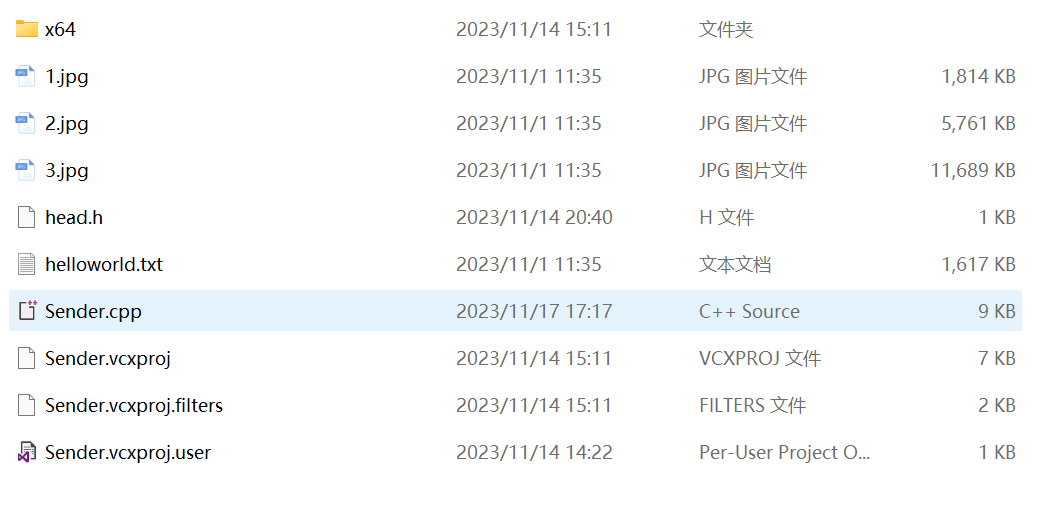
\includegraphics[width=0.6\textwidth]{img/测试文件.png}
    \caption{测试文件}
\end{figure}
按照代码中设置的端口号,Sender端口为5000,Router端口为6000,Receiver端口为7000。设置丢包率为3\%,延时为5ms。配置路由程序如下图所示:
\begin{figure}[H]
    \centering
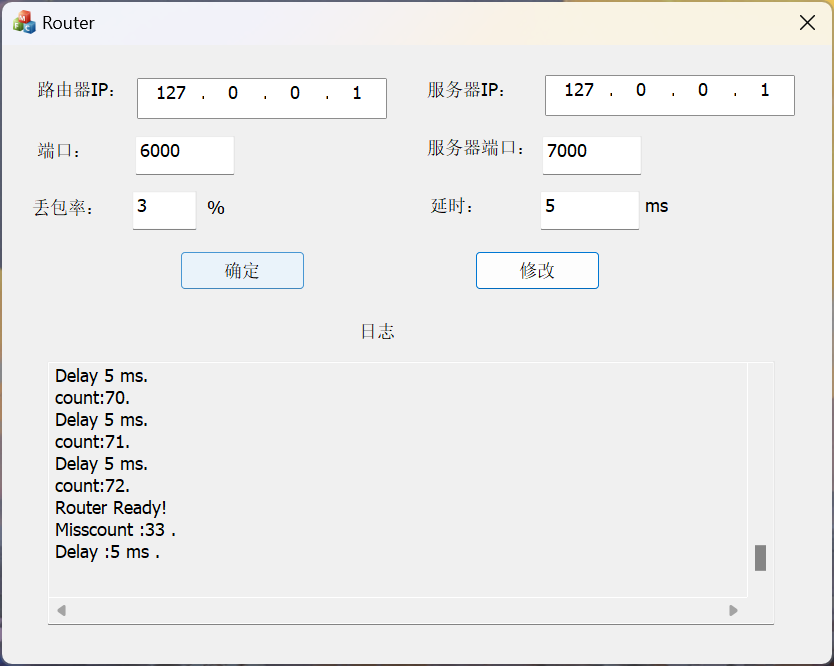
\includegraphics[width=0.4\textwidth]{img/路由程序界面.png}
    \caption{路由程序界面}
\end{figure}
先后打开Receiver.exe和Sender.exe,初始化界面如下:
\begin{figure}[H]
    \centering
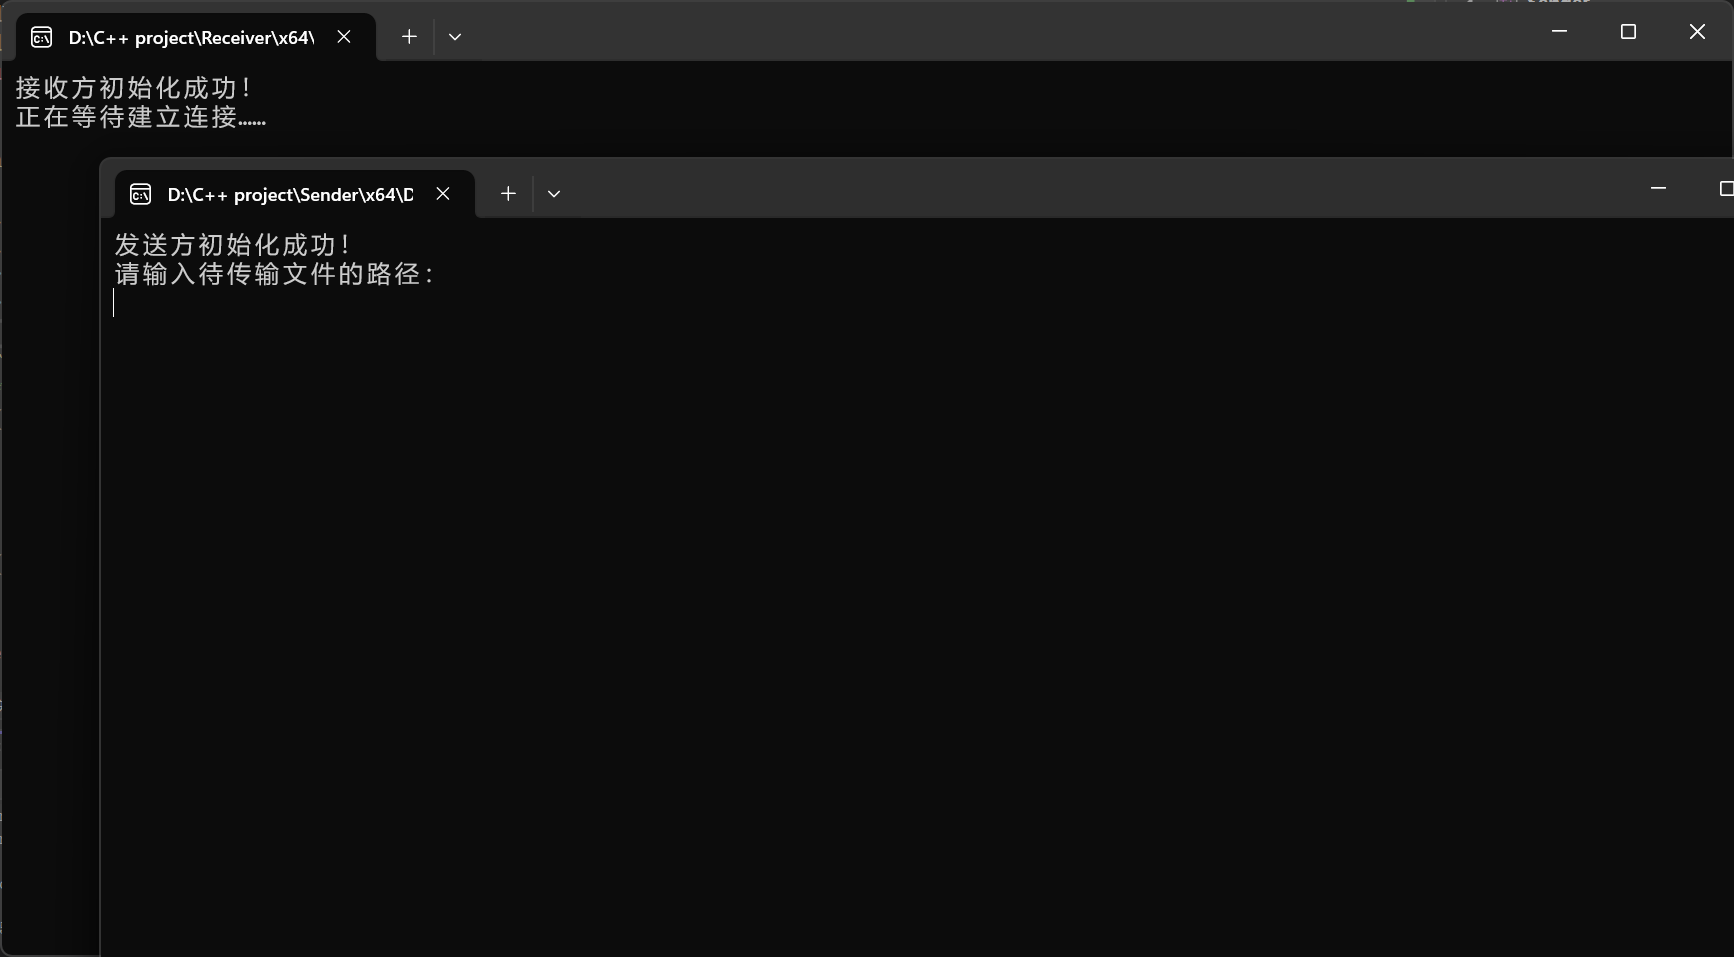
\includegraphics[width=0.8\textwidth]{img/初始化界面.png}
    \caption{初始化界面}
\end{figure}
输入路径$./helloworld.txt$,按下回车开始传输
\begin{figure}[H]
    \centering
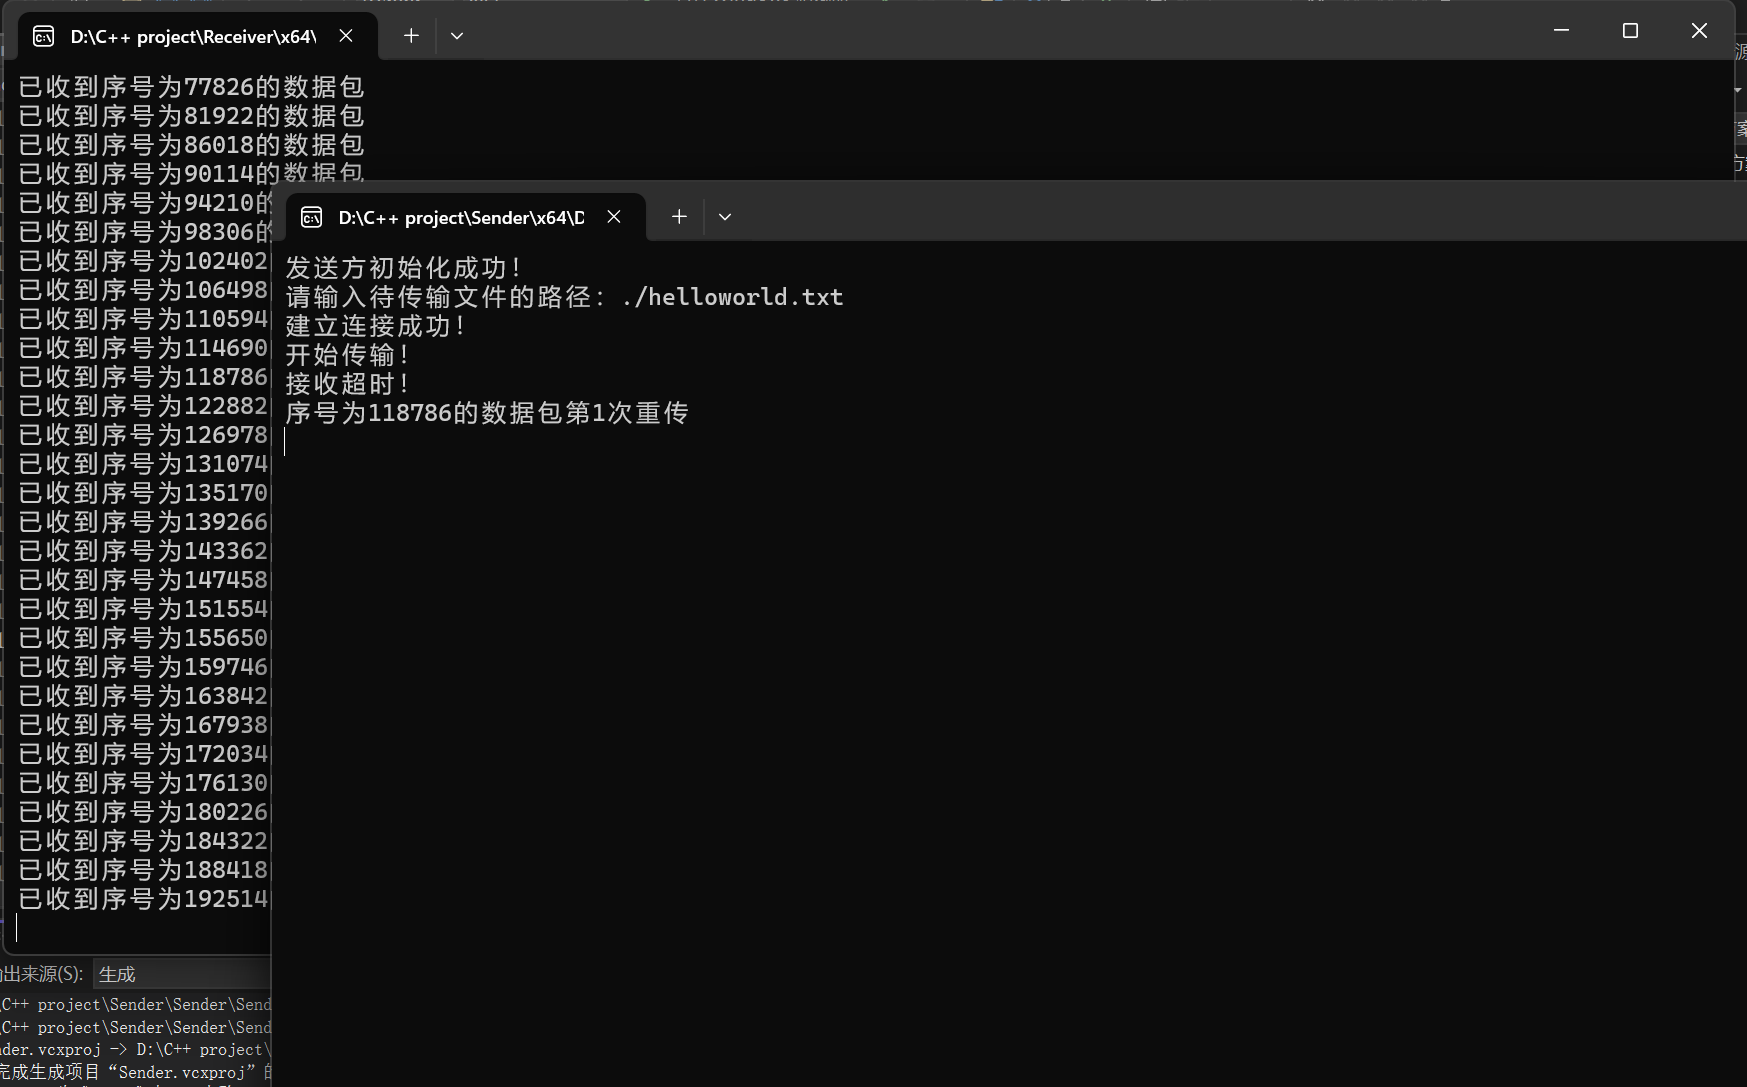
\includegraphics[width=0.8\textwidth]{img/传输过程1.png}
    \caption{传输过程1}
\end{figure}
可以看到,接收端源源不断地输出收到数据包信息,发送端输出重传信息,符合实验预期。同时路由器在不断输出日志信息,说明路由器成功完成丢包和延时的操作。
\begin{figure}[H]
    \centering
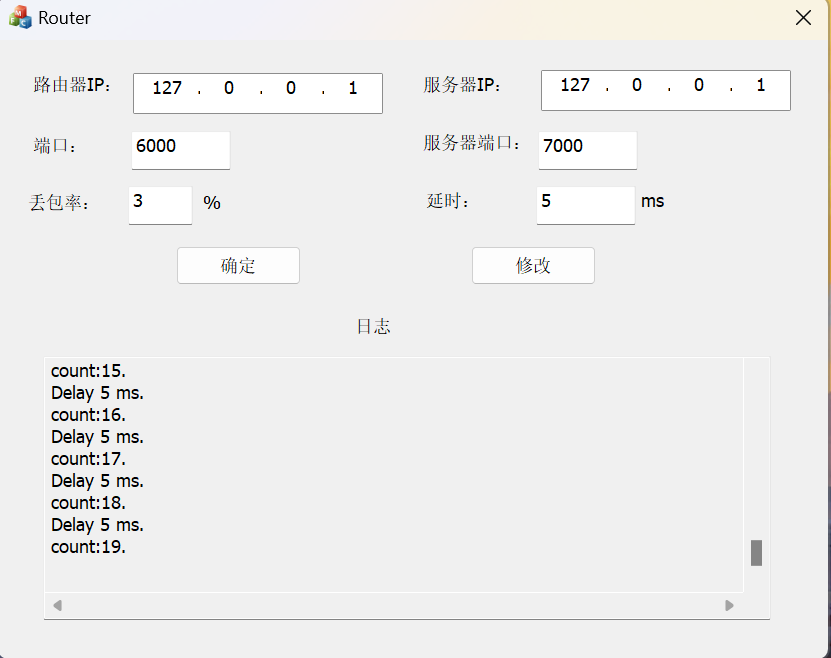
\includegraphics[width=0.8\textwidth]{img/路由器日志输出.png}
    \caption{路由器日志输出}
\end{figure}

\begin{figure}[H]
    \centering
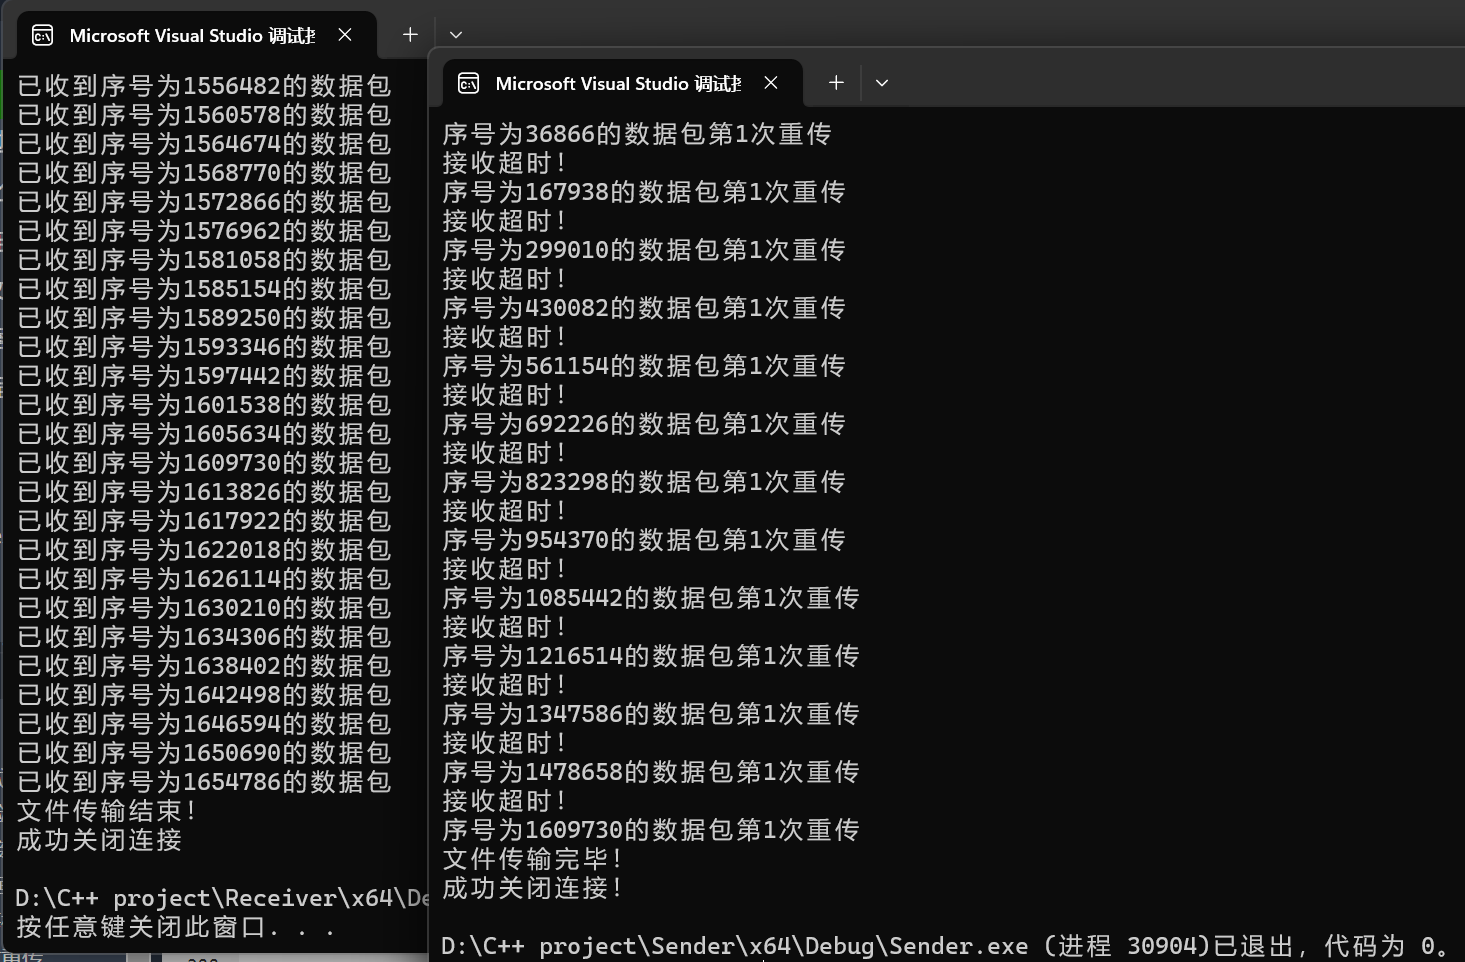
\includegraphics[width=0.8\textwidth]{img/传输过程2.png}
    \caption{传输过程2}
\end{figure}
传输结束后,双方正确输出提示语,并且成功关闭连接。
\begin{figure}[H]
    \centering
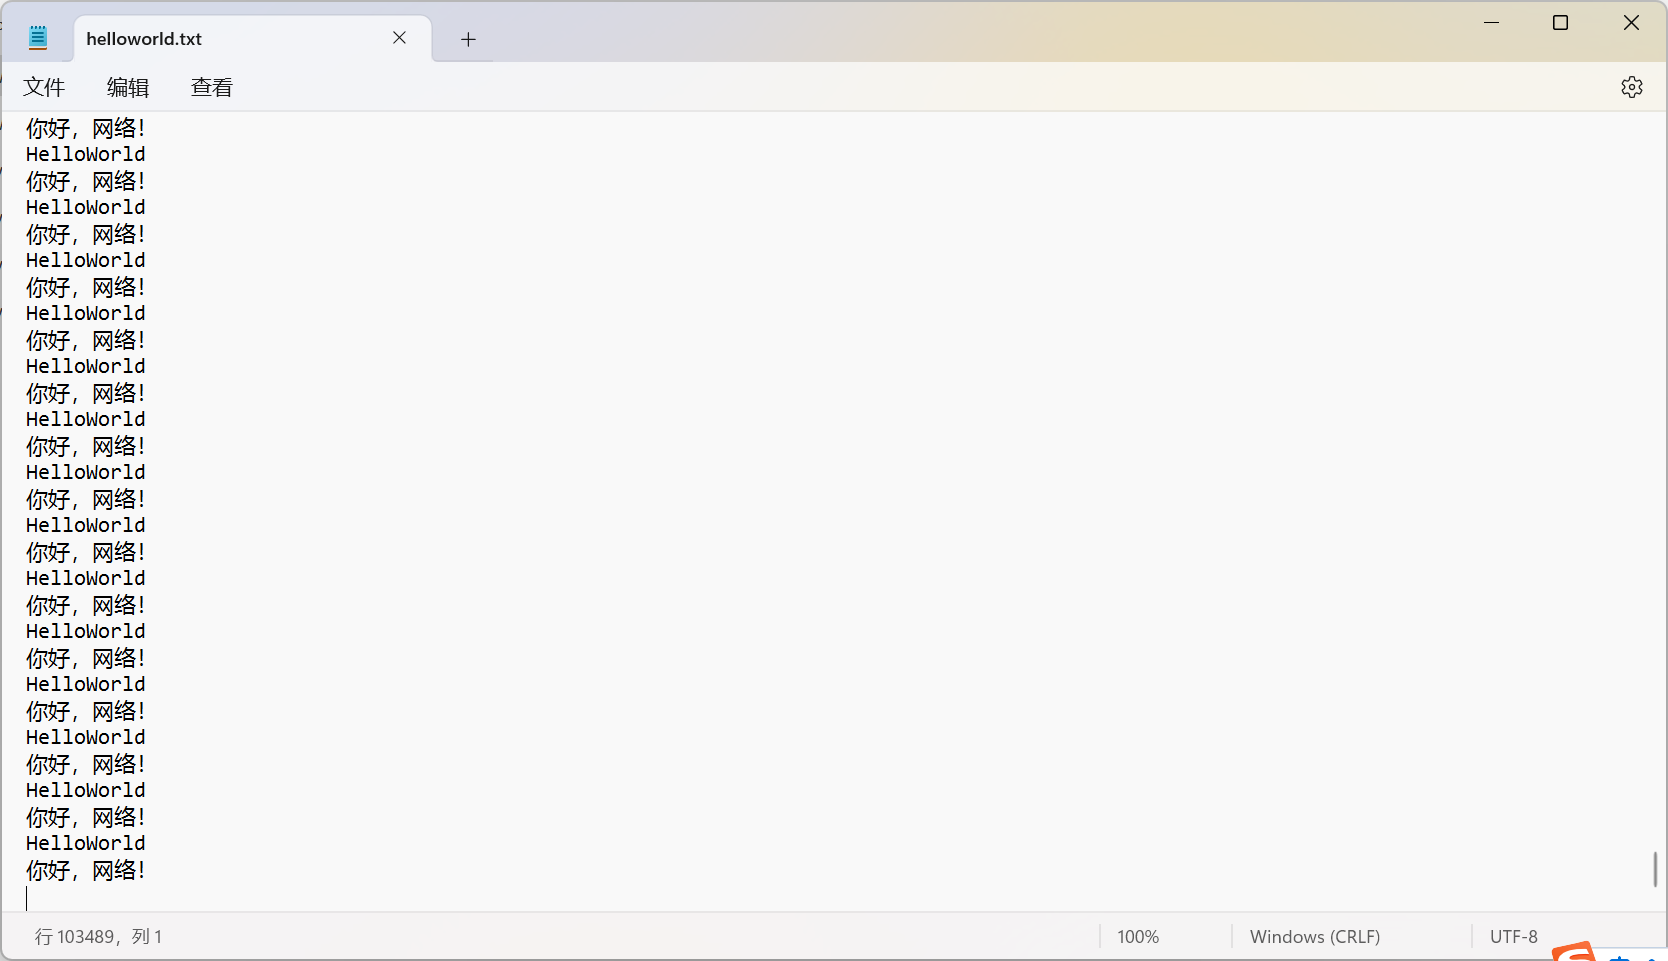
\includegraphics[width=0.8\textwidth]{img/实验结果.png}
    \caption{实验结果}
\end{figure}
打开Receiver的目录,可以看到输出的文件,同时文件大小与源文件大小相同。txt文件的行数也与原始文件相同。接下来传输$1.jpg、2.jpg、3.jpg$,都能在Receiver目录下成功得到输出的图片,同时图片大小与原图相同。结果如下:
\begin{figure}[H]
    \centering
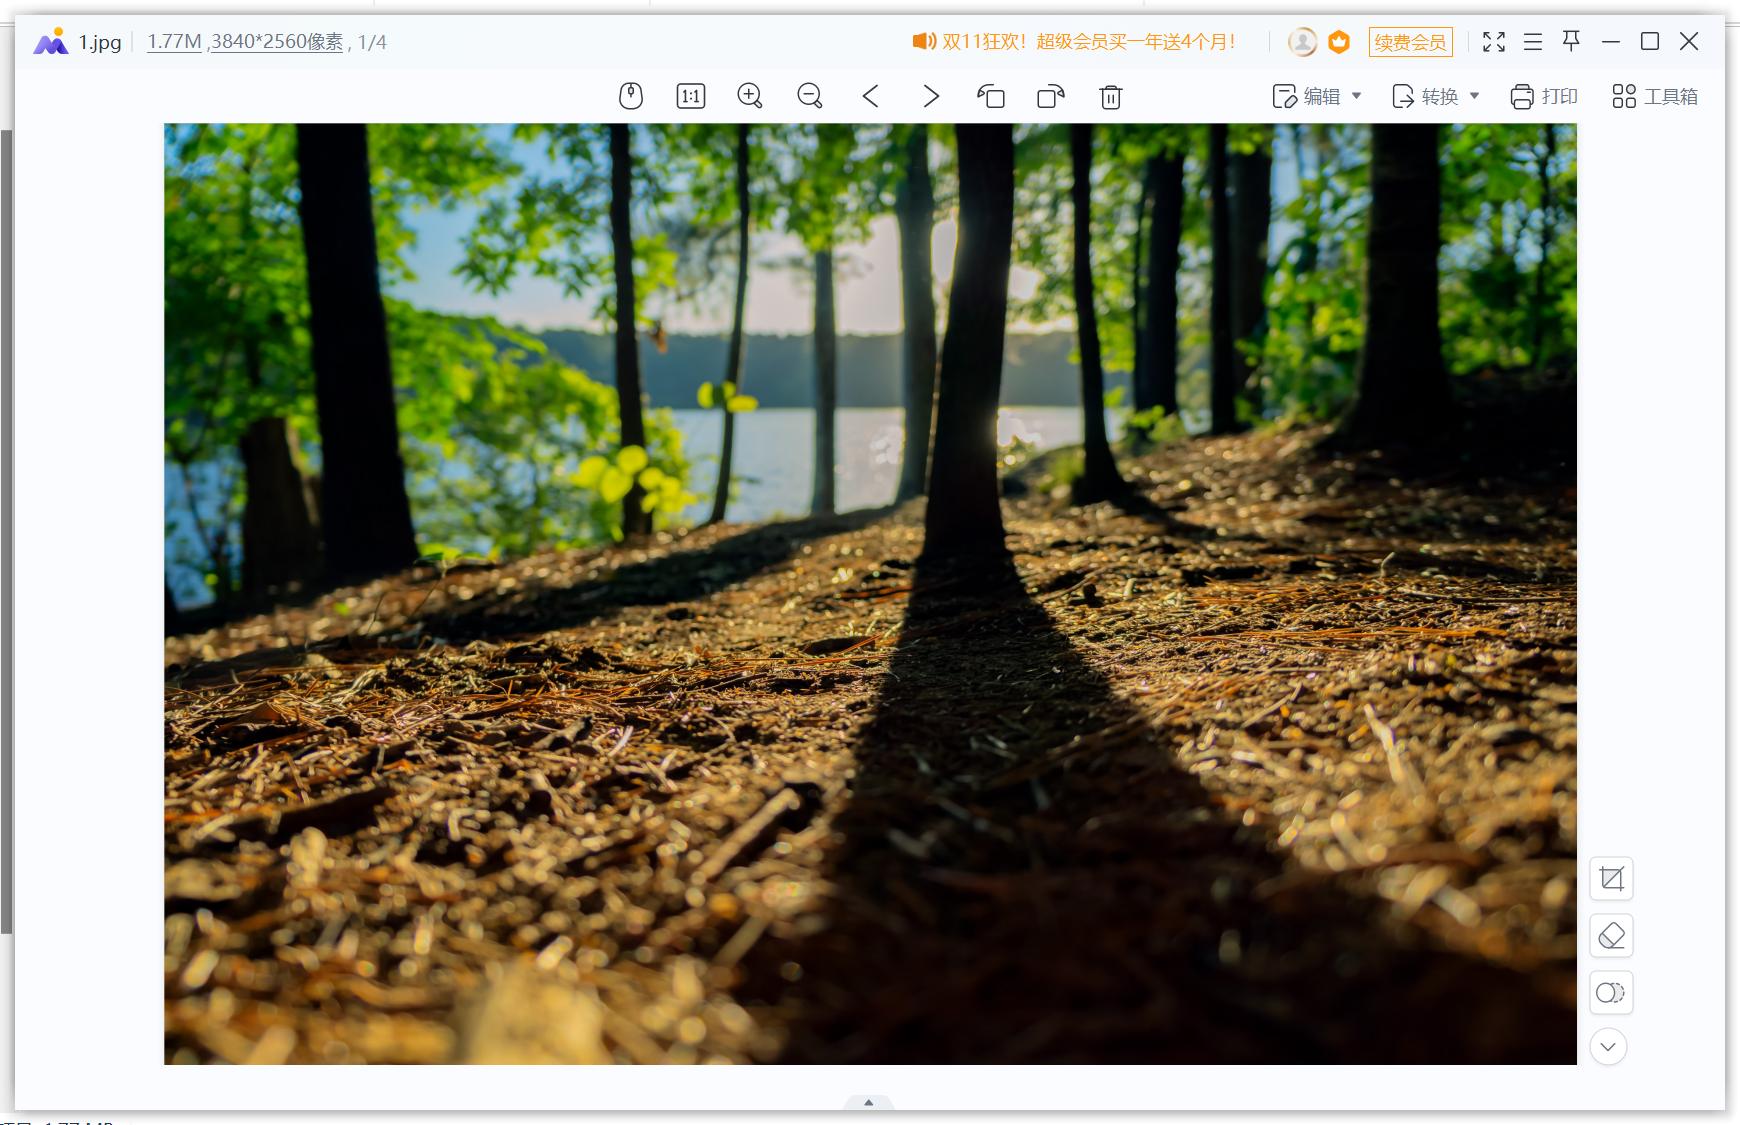
\includegraphics[width=0.8\textwidth]{img/图片1.png}
    \caption{图片1}
\end{figure}
\begin{figure}[H]
    \centering
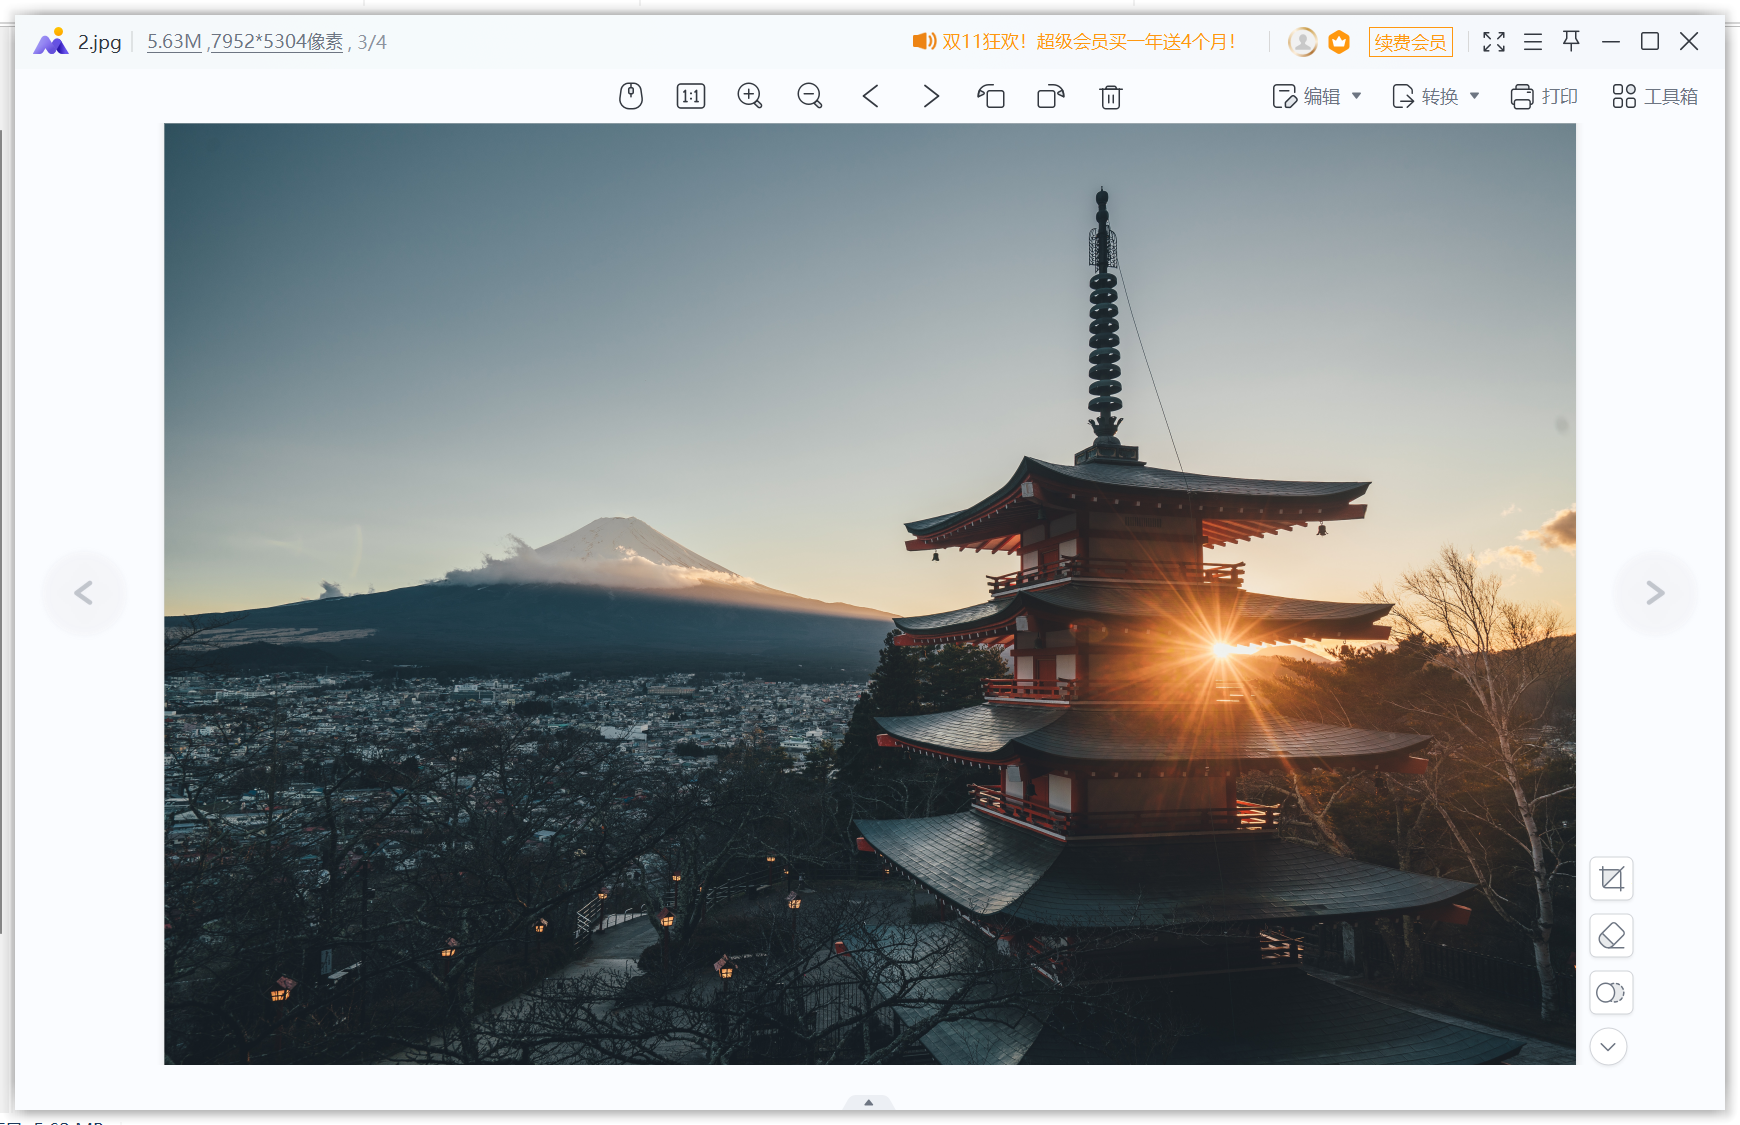
\includegraphics[width=0.8\textwidth]{img/图片2.png}
    \caption{图片2}
\end{figure}
\begin{figure}[H]
    \centering
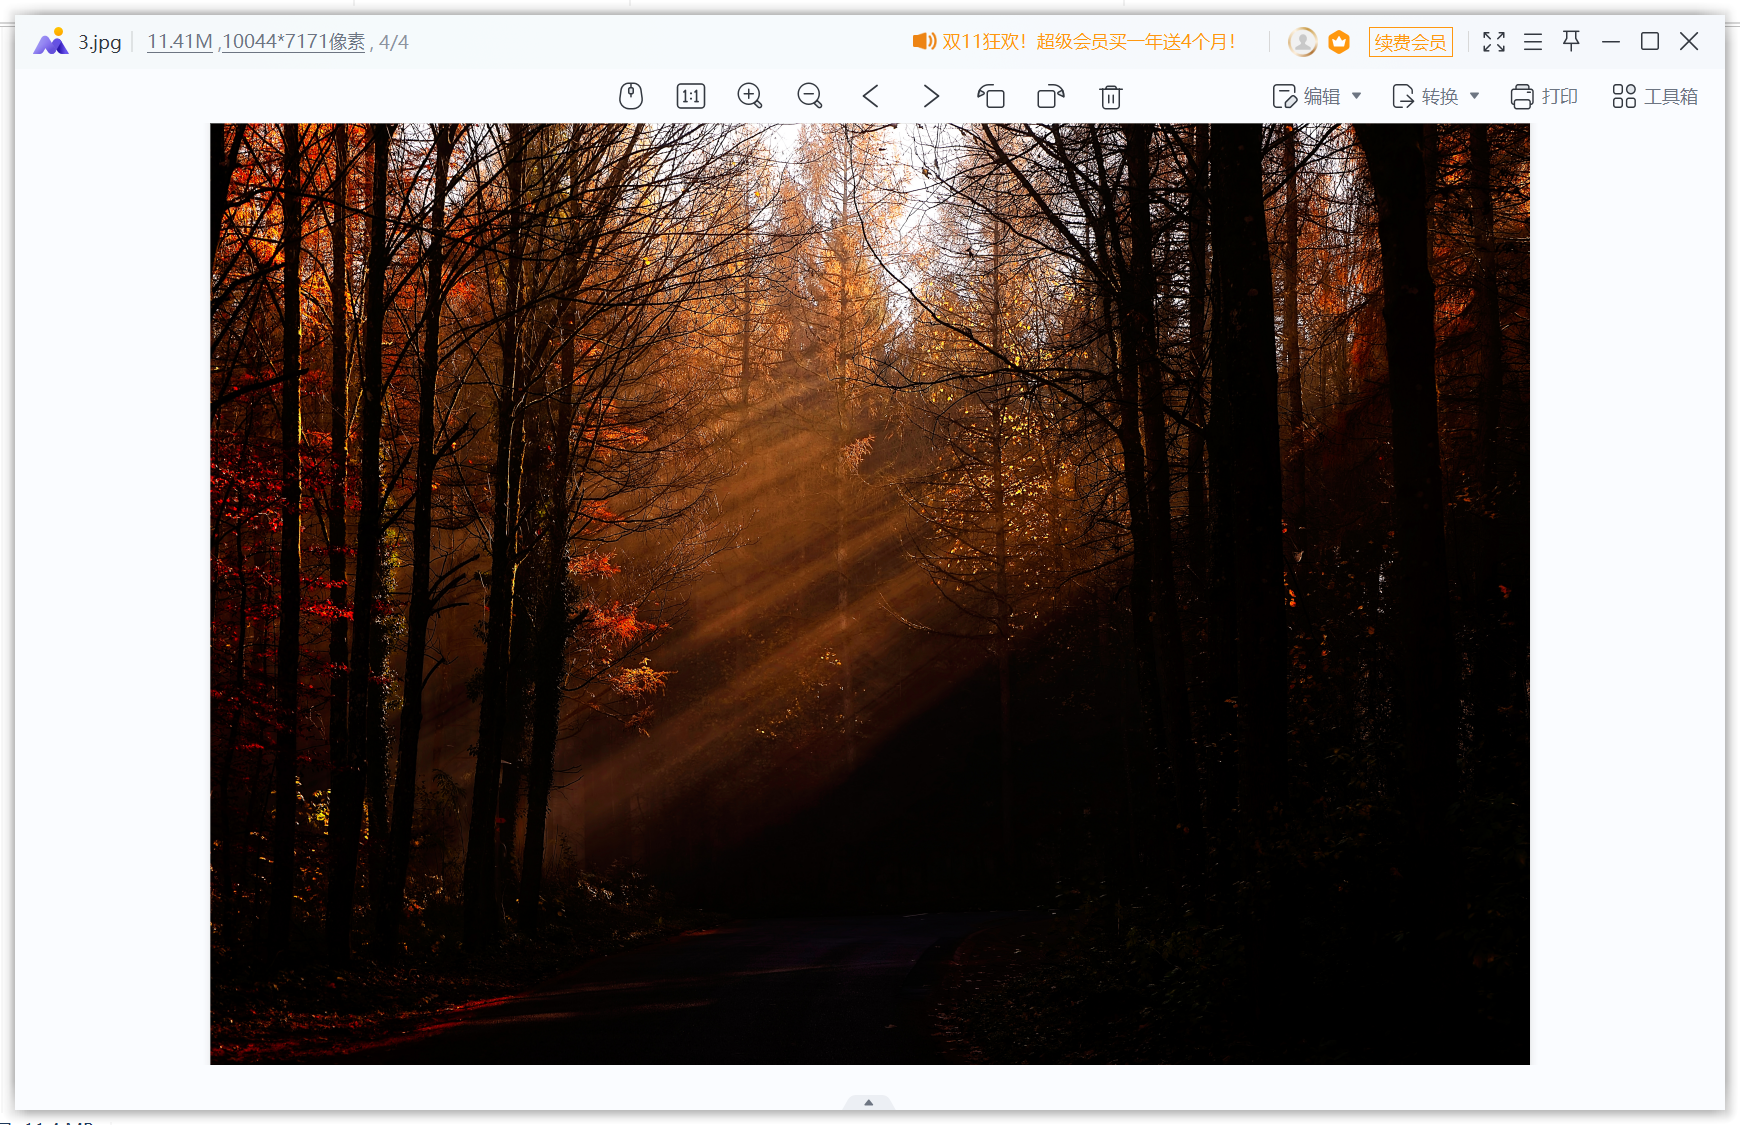
\includegraphics[width=0.8\textwidth]{img/图片3.png}
    \caption{图片3}
\end{figure}
在实验前,我们利用基础UDP服务传输$1.jpg$,发现文件大小小于源文件大小,说明传输过程中发生了丢包,也验证了UDP传输不可靠的特点。
\section{思考\&总结}
本次实验利用UDP的Socket编程实现了可靠数据传输。但在实验中,发现可靠性虽然得到了保障,但传输的性能和效率方面还有巨大的优化空间。在之后的实验中,会改用更加复杂的滑动窗口机制来代替停等机制,在失序数据包的处理上也会用选择重传机制来代替直接丢包的操作,提高传输性能和效率。
\end{document}
